\section{Design}
The design considers the context in which the problem exists and the design of each system and subsystem necessary to visualize and realize a possible solution to solve the problem.

The nature of the system exists primarily in the software domain.
As such, a suitable design architecture is postulated by the C4 model.
This model breaks down the system architecture into different layers of complexity, from a generic high-level system overview down to low-level software abstractions.\cite{vazquez2020c4}

Low-level abstractions are realized with \ac{uml} diagrams. \Ac{uml} diagrams detail the members and methods belonging to classes, and the relationships between those classes in an object-oriented codebase. \cite{petre2013uml}

\subsection{System context and base requirements }
Figure \ref{fig:system_context} depicts the system context in the problem domain.
Project specifications have identified two parties expected to utilize the system - truck drivers and fleet managers.
Identified requirements on the solution dictate that truck drivers will use an android application to log data on the system.
In addition, fleet managers must view the logged data and manipulate their fleets via a web application running in a browser.

\begin{figure}[H]
\centering
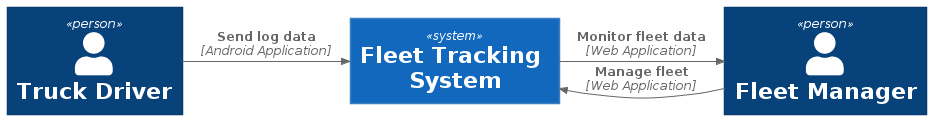
\includegraphics[width=6in]{../diag/system_context.png}
\caption{System Context Diagram}
\label{fig:system_context}
\end{figure}

\begin{figure}
\centering
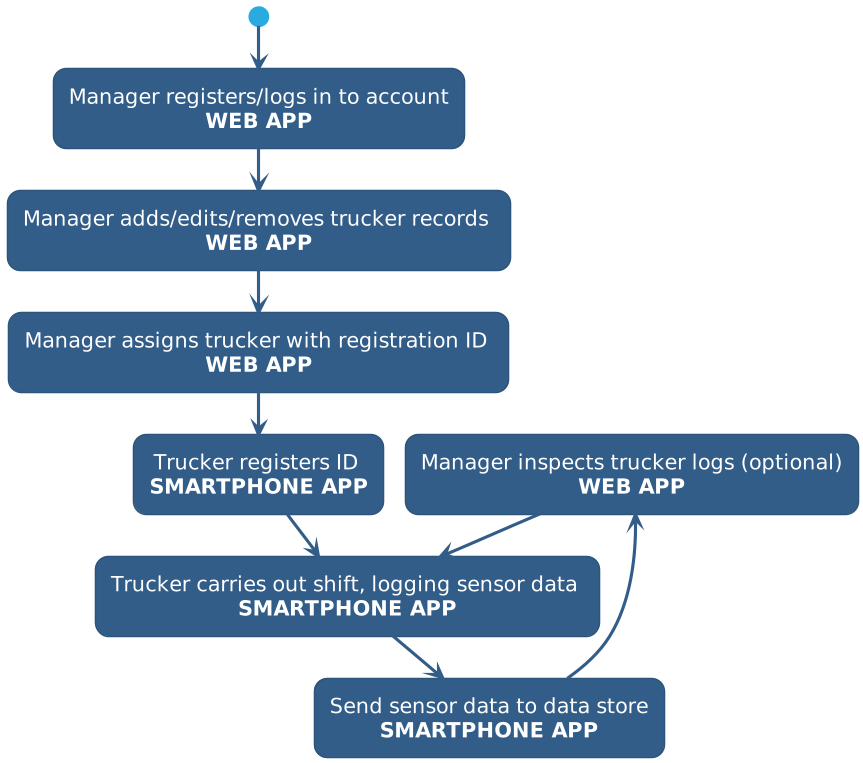
\includegraphics[scale=0.40]{../diag/high_level_activity.png}
\caption{System Lifecycle - High Level}
\label{fig:high_level_activity}
\end{figure}

The high-level life cycle view of the fleet-tracking system design is depicted in figure \ref{fig:high_level_activity}.
This life cycle view gives a broad indication of how the system is expected to work for a user.
Only front-end components of the system are considered to clarify exactly how users will interact with the system.

Managers are required to perform initial configuration, including adding trucker identity records to a data store.
After this, truckers may connect to the system and perform their work while allowing their smartphone applications to track the required sensor data. 
This data is then relayed to the system, in which managers may analyze and inspect data logs.

\subsection{Contained subsystems and choice of technologies}
The second level of the C4 model identifies the choice of technologies to be utilized to realize the fleet tracking system.
The fleet-tracking system is divided into mostly-independent containers, as depicted in figure \ref{fig:container}.
Each container is a standalone process which makes calls to other processes in the system.
The main choice of software tools are identified for each container.

Truckers will make use of an android data-logging application to fetch the various sensor data, and securely transmit this data via an \ac{ssl} connection.
The \ac{io} server, implemented in C++, will listen for multiple asynchronous connections from the android application and relay the data to a MySQL database.
A web application, realized with Microsoft's ASP.NET framework fetches the data and allows the fleet manager to view the whereabouts of each member in his/her fleet.
\begin{figure}[H]
\centering
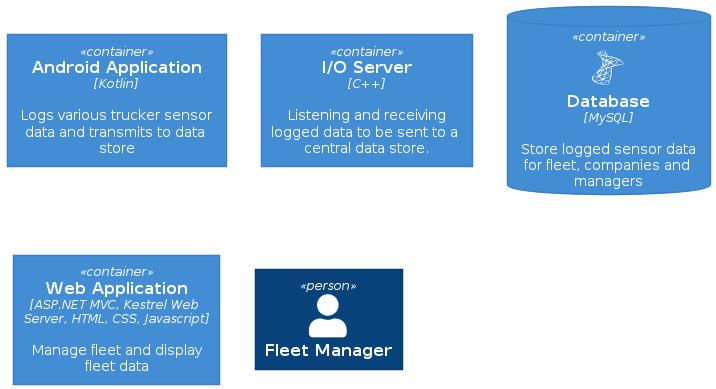
\includegraphics[width=6in]{../diag/container.png}
\caption{Container Diagram - Fleet tracking system}
\label{fig:container}
\end{figure}

\subsubsection{Choice of \ac{rdbms}}
The entire system revolves around the effective abstraction and manipulation of logged fleet data.
MySQL is chosen as the \ac{rdbms} to realize a relational database model, as it is highly performant and reliable.
Other \ac{rdbms}s (such as Microsoft SQL Server, PostgreSQL) offer comparable performance, but MySQL is chosen for familiarity.

\subsubsection{Android Application}
The smartphone application is written for the Android \ac{os}, due to its cost benefits and larger market share.

Kotlin is the language of choice to write the android application due to its simplicity, modern powerful feature set and mainstream Google support.
Kotlin runs on the \ac{jvm} (as does Java) but offers a cleaner development experience with modern features such as coroutines, flows and less verbosity (and therefore less "code smells").
Common Java classes may be called within Kotlin code, allowing for the legacy Java libraries to be integrated with modern Kotlin code.

Truckers must receive an initial code from their managers' to register their devices.
Sensor readings are taken every two minutes, and stored into a lightweight database.
Finally, a connection is attempted with an \ac{io} server. If available, the database contents is emptied into via the \ac{io} server to the central system database.

\subsubsection{\Ac{io} Server}
C++ is chosen for the \ac{io} server, due to its high performance capabilities.
The \ac{io} server needs to listen and allow multiple asynchronous connections, during which log data is transmitted to the database.

\subsubsection{Web Application}
Web applications consist of a backend (running on a server) component, and serves content to the frontend component (rendered on a browser).

Many web frameworks can be used to build effective and powerful web applications.
Frameworks such as Node.js, Express, Django, Rails, Spring all offer a feature rich experience.
Choice often depends on preference.
Microsoft's ASP.NET web framework is chosen as it offers great performance, and is familiar.

\subsection{Subsystem components and Design}
Each container in figure \ref{fig:container} is subdivided into several core software components necessary to achieve the desired outcomes.
This is depicted through container diagrams, which makes up the third level of the C4 model.

\subsubsection{Android Application - lifecycle and software abstractions}
\begin{figure}
\centering
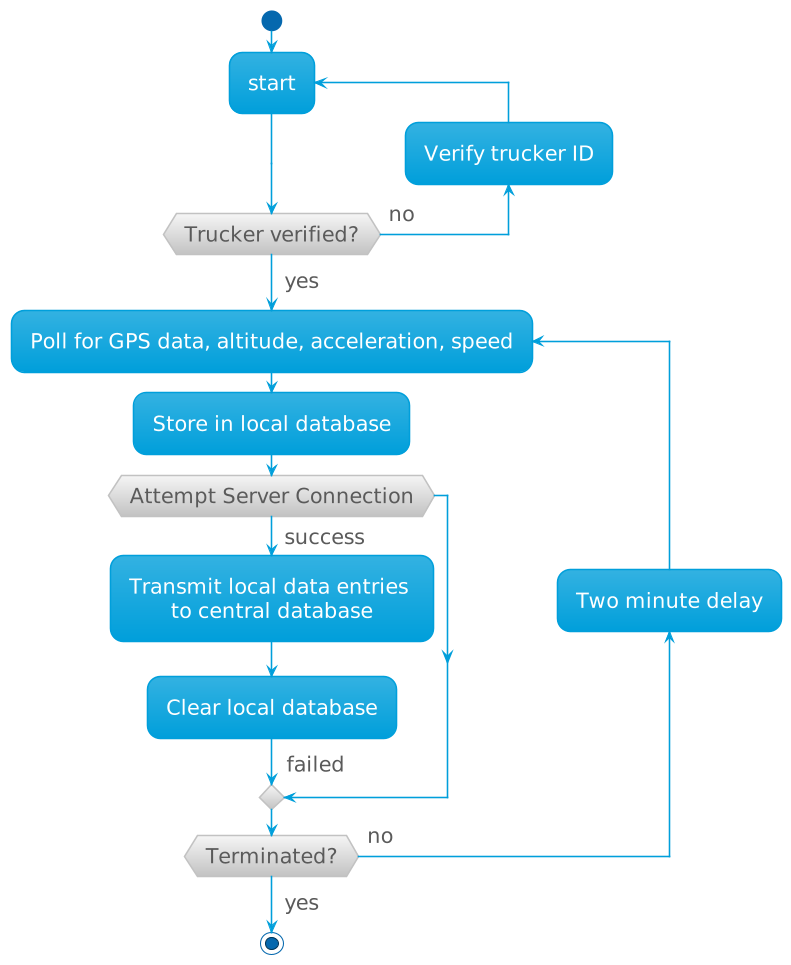
\includegraphics[scale=0.4]{../diag/android_activity.png}
\caption{Life-cycle - Android Application}
\label{fig:android_activity}
\end{figure}

The life cycle of the Android application is depicted in figure \ref{fig:android_activity}.
Initially, a check is performed to confirm that the trucker \ac{id} is in the central database, and is not duplicated.
If this \ac{id} is not valid, the trucker must request a valid \ac{id} from the fleet manager.

After this, the usual logging process is continued.
Data is polled from the available sensors and stored in a local database.
A connection is attempted with the \ac{io} server and the local database entries are transmitted to the server.
Upon successful transmission, the local database is cleared.
However, if a connection fails, the local database is not cleared.
This process loops continuously loops every two minutes.
 
\begin{figure}
\centering
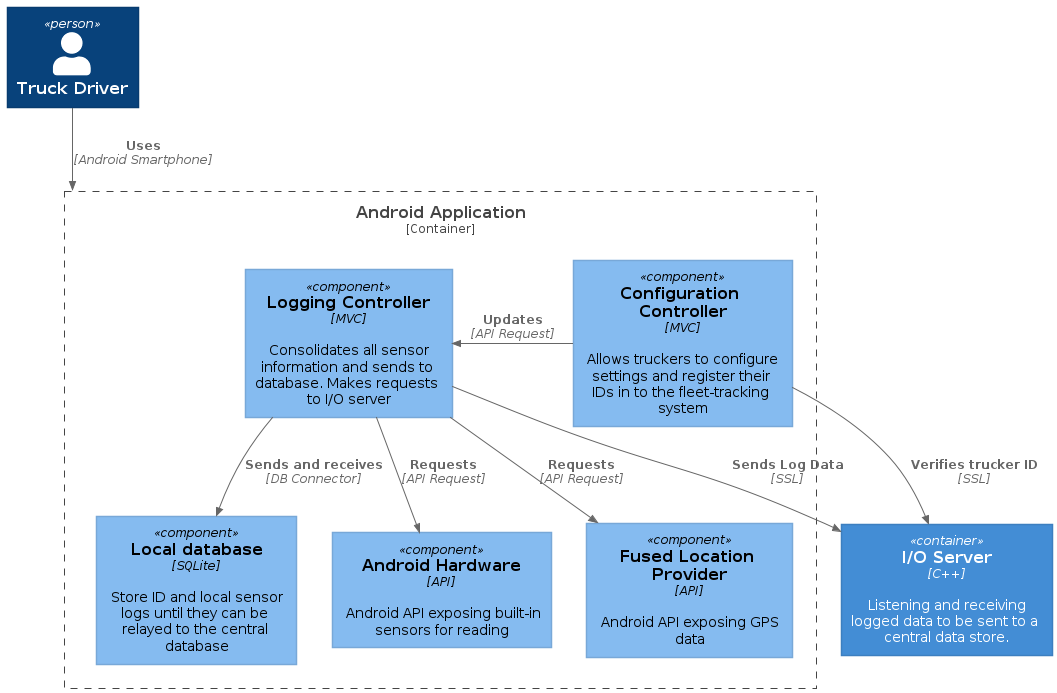
\includegraphics[width=6in]{../diag/android_component.png}
\caption{Component Diagram - Android Application}
\label{fig:android_component}
\end{figure}

The android application is designed with the \ac{mvvm} design pattern (detailed in figure \ref{fig:mvvm_layout}).
Figure \ref{fig:android_component} details software components (classes) that are clearly represented in the source code.
The application is targeted to support Android version 4.4 onward.
This allows for the application to run on 99.6\% of Android devices.

\begin{enumerate}
\item \textbf{Main Activity}\\
The main activity renders the application's main user interface to the user.
This component mainly implements \Ac{ui}-handling logic, with callbacks which are primarily event-driven (when users press buttons for example).
\item \textbf{Main View Model}\\
Activities have short lifetimes and are often recreated when users switch between applications or tilt their screens.
Due to this, a manager class is necessary to ensure data is persisted - this is achieved by the view model.
\item \textbf{Tracking Service}\\
The tracking service is toggleable service which runs in the background as a foreground service.
It polls acceleration and location data via interfaces made available in the Android \ac{api}.
It runs without requiring the main activity to be open on the user's screen.
\begin{enumerate}
\item \textbf{Fused Location Provider \ac{api}}\\
The Android \ac{api} provides the \textit{Fused Location Provider} for the purposes of accessing location data according to required settings.
The \ac{api} provides callbacks which can be hooked into for storing location data, at an adjustable interval.

\item \textbf{Sensor Manager}\\
The sensor manager provides callbacks for reading data from the various sensors (including accelerometers).
The \textit{Linear accelerometer} is a "composite" sensor which relies on magnetometers or gyroscropes, in addition to the accelerometer to "zero" out the acceleration due to gravity.
This is provided by the Android \ac{api}.
Devices without Linear acceleromters require signal processing to remove the gravitational component. However, this processing is very limited in accuracy.

Acceleration will only be logged in devices with linear accelerometers.
\end{enumerate}
\item \textbf{Main Repository}\\
Multiple components require performing \ac{io} operations.
To avoid repetition and prevent conflicts, the main repository performs these operations.
It exists as a singleton and is injected into calling objects with \ac{di}.
\item \textbf{Room - Object Relational Mapper}\\
Android's room abstraction layer provides a data class abstraction of data stored in the SQLite database.
This abstraction makes it easier to work with data in language-specific data structures.
Room provides a \ac{dao} to the main repository for database operations.
\item \textbf{SQLite database}\\
SQLite is a lightweight go-to database provider for Android applications.
It is ideal for storing medium to small sized volumes of data.
\item \textbf{Server Connector}\\
The server connector provides \ac{ssl} socket communication with the central \ac{io} server.
Request objects are serialized into text data streams for transmission.
Likewise, server responses are deserialized into response objects and handled appropriately.
\item \textbf{Shared Preferences}\\
Android's \textit{SharedPreferences} library provides an \ac{api} for the purposes of reading/writing key value data in a file on disk.
This is used for storing user configuration, such as identity and upload preferences, which aren't appropriate for a database.
\end{enumerate}

These components are necessary for realizing a modular, extendable application.

\pagebreak
\subsubsection{\Ac{io} Server}
The typical life cycle view of the \ac{io} server is depicted in figure \ref{fig:IO_activity}.
A secure connection must be made due to the sensitive nature of \ac{gps} data.
\begin{itemize}
\item A session is assigned for the lifetime of the communication, which handles the three-way \ac{ssl} handshake, ensuring the client trusts the server. The incoming payload is decrypted.
\item A request handler parses (and deserializes) the decrypted payload, which queries the database to generate an appropriate serialized response.
\item The response is sent back to the client and the session is terminated.
\end{itemize}

The popular C++ library, \textit{asio} can implement the above workflow in an asynchronous manner.

\begin{figure}
\centering
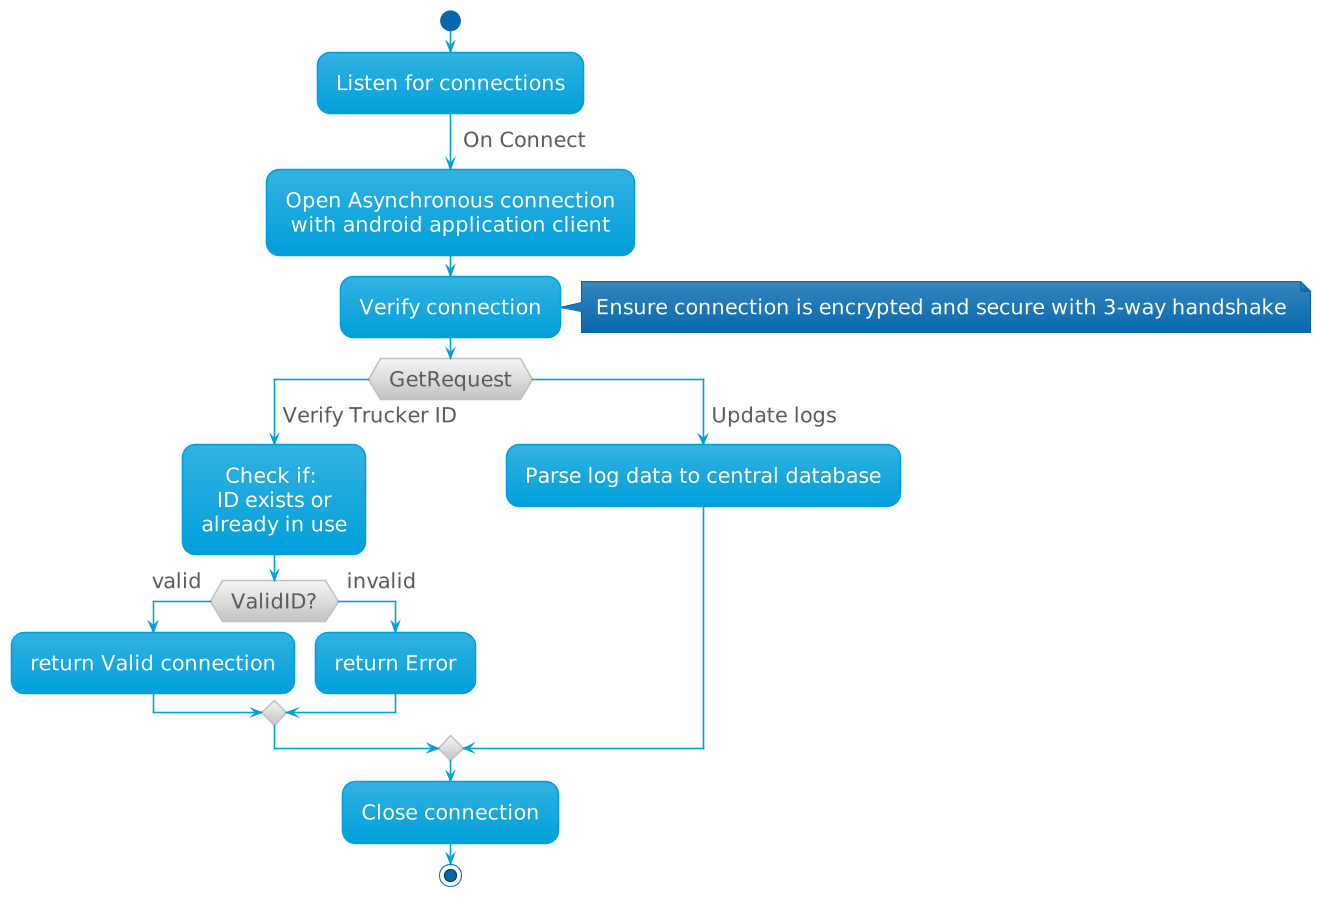
\includegraphics[width=6in]{../diag/IO_activity.png}
\caption{Life cycle - \Ac{io} Server}
\label{fig:IO_activity}
\end{figure}

\begin{figure}[H]
\centering
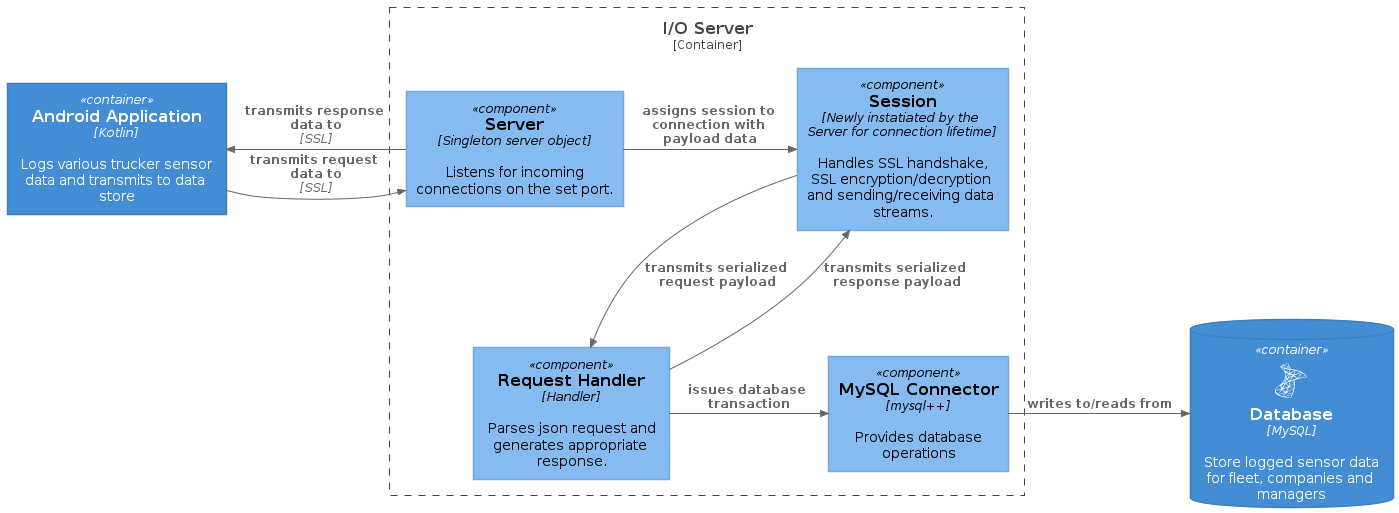
\includegraphics[width=6in]{../diag/IO_component.png}
\caption{Component Diagram - \Ac{io} Server}
\label{fig:IO_component}
\end{figure}

Figure \ref{fig:IO_component} depicts the software abstractions and program structure used to realize the \ac{io} server.
The codebase clearly contains these low-level abstractions.
\begin{enumerate}
\item \textbf{Server}\\
The server object listens for incoming \ac{tcp} connections.
Upon receiving a connection, a new session is instantiated to handle to communication.
\item \textbf{Session}\\
The session performs the necessary encryption, decryption and three-way handshake required for the \ac{ssl} protocol.
The session reads in and writes out the serialized payload on the socket.
\item \textbf{Request Handler}\\
The request handler performs serialization and deserialization.
It processes the request and queries the database appropriately.
\item \textbf{MySQL Connector}\\
An interfacing object to the MySQL database.
\end{enumerate}

\pagebreak
\subsubsection{\ac{json} protocol}
Figure \ref{fig:json_protocol} depicts the structure of the protocol used for communication between the \ac{io} server and the android client.
The communication follows a \ac{rest}ful structure, which is common for web communications.
That is, communication requires no knowledge of intermediate state.
One request is enough to complete the required transactions, after which an appropriate response is sent back to the client.

\begin{figure}[H]
\centering
    \subfigure[Request payload]
    {
        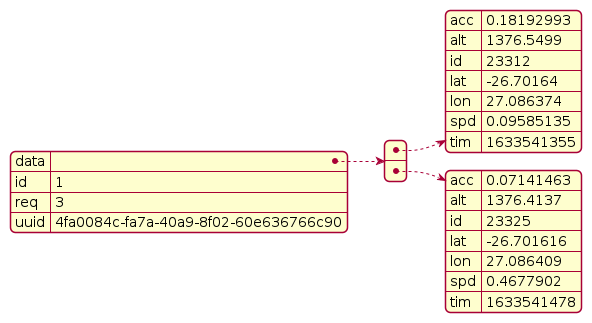
\includegraphics[scale=0.5]{../diag/json_request.png}
        \label{fig:json_request}
    }
    \subfigure[Response payload]
    {
        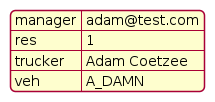
\includegraphics[scale=0.5]{../diag/json_response.png}
        \label{fig:json_response}
    }
\caption{\Ac{json} protocol}
\label{fig:json_protocol}
\end{figure}


\begin{itemize}
\item The client makes a request in \ac{json} form, as shown in figure \ref{fig:json_request}.
It contains \ac{id} information about the client, a request code and any payload data (typically tracking data). Possible requests include verifying \ac{id}, sending log updates and registering new \ac{id}s.
\item The server appropriately handles the request (based on request code) and generates an appropriate response. Usually the response will just contain the response code, but it may sometimes carry extra information (as seen in figure \ref{fig:json_response}).
Responses can return a fail, ok, invalid credential, database connection error or parsing error status.
\end{itemize}

 This communication is realized through \ac{ssl} sockets over the network.

\pagebreak
\subsubsection{Web Application}
The web application is modeled with the \ac{mvc} design pattern, which allows for following \ac{soc} principles.
Backend logic is realized in C\# using Microsoft's \textit{ASP.NET} framework.
Web pages are generated with a combination of C\#, JavaScript and \ac{html} styled with \ac{css}.

\begin{figure}[H]
\centering
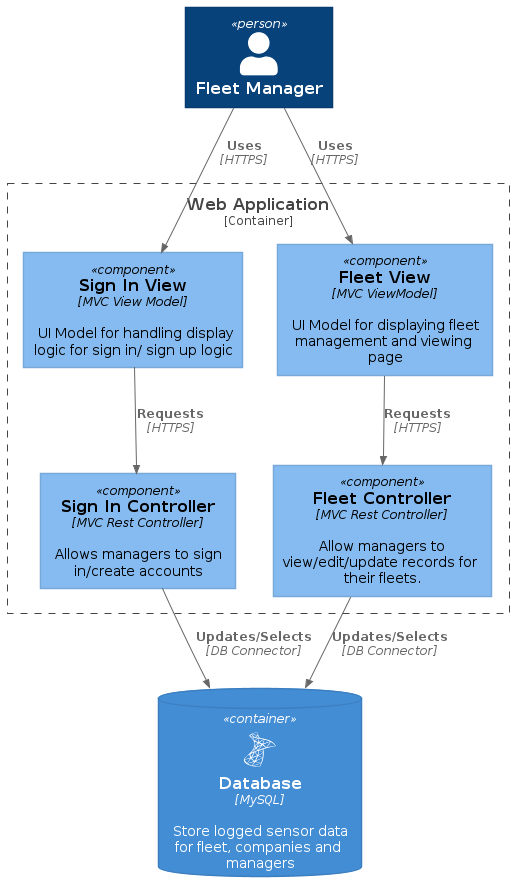
\includegraphics[width=6in]{../diag/webapp_component.png}
\caption{Component Diagram - Web Application}
\label{fig:webapp_component}
\end{figure}

Figure \ref{fig:webapp_component} depicts the architectural arrangement of the web application.
\begin{enumerate}
\item \textbf{ASP.NET Identity Views and Controller}\\
Microsoft provides a professional library for handling user access, known as \textit{ASP.NET Identity}.
This library handles logic for user registration, signing in and account editing.
In addition, there is support for email verification and two-factor authentication.
Identity also implements logic for restricting access to pages, ensuring managers can only view data related to their fleets'.

\item \textbf{DB Context and MySQL database}\\
Microsoft's \textit{Entity Framework} provides the abstraction of data as 'entites' to be represented by models (data classes in code).
This makes for easier interaction with data in code.
The back-end database in use is MySQL.

\item \textbf{Fleet Models}\\
The Fleet Models are a set of data classes used for the abstraction of data entities in code.
They allow for the easy passing of data from controllers to views.
An extra view model class is used for viewing truckers.
Since viewing truckers requires extra processing of trucker information logs, an extra class is utilized to handle this processing.

\item \textbf{Fleet Controller}\\
User interactions from any of the fleet views results in \ac{http} requests issued to the Fleet Controller.
The Controller has multiple methods for handling different \ac{http} requests.
Upon receiving a routed request, it selects the appropriate method and queries the appropriate fleet data from the database abstraction layer.
The results of the query are populated into one of the models, and the model is returned to the view.

\item \textbf{Fleet Views}\\
Multiple views are returned by the Fleet Controller depending on request, and act as the \ac{ui} component visible to the user.
Each view only handles the necessary logic required for displaying data returned as a model from the controller.
The \ac{ui} is rendered as \ac{html}, with backend C\# logic utilized to dynamically render view components, such as tables.
Additional \ac{ui} logic is realized with JavaScript.

\begin{enumerate}
\item \textbf{Index}\\
The Index view displays a list of all truckers registered by the manager.
It provides an interface for resetting each trucker's Android \ac{id}.

\item \textbf{Add Trucker}\\
The "Add Trucker" page provides an \ac{html} form for the purposes of adding trucker's to the fleet.
Details about the trucker such as name and vehicle number can be added.

\item \textbf{Set Rules}\\
The "Set Rules" page allows the manager to define custom rules defining unacceptable driving behavior, including maximum speed and acceleration.

\item \textbf{View Trucker}\\
The "View Trucker" page displays details about the trucker's activities for an adjustable time period.
A table is used to group location data into individual trips.
This table is generated by means of a grouping algorithm to segment the driver's activities into separate trips, and includes information such as waiting time, average speed and indications of any rule breaks.

In addition, each trip is drawn in a map using the \textit{Google Maps JavaScript \ac{api}}.
This provides a neat visual representation of Trucker activities.

\item \textbf{View Trip}\\
The "View Trip" page allows for detailed statistical analysis of individual trips.
It provides percentile analysis and graphs showcasing the trucker's speed, acceleration and altitude.
\end{enumerate}

\end{enumerate}

\pagebreak
\subsubsection{MySQL Database and Entity relationships}
The central backend \ac{rdbms} used is MySQL.
A relational data structure is utilized, as shown in figure \ref{fig:erd}.
Relational modeling allows for logical structuring and integrity of the data.

\begin{figure}[H]
\centering
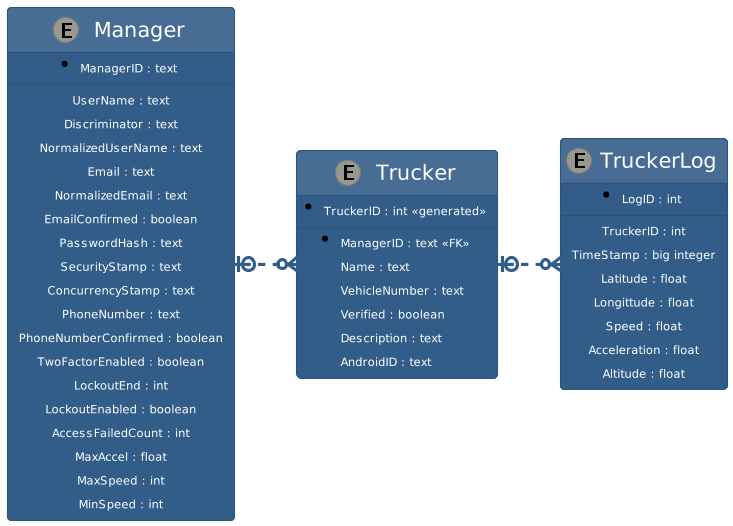
\includegraphics[scale=0.5]{../diag/erd.png}
\caption{Fleet Tracking System - Entity Relationship Diagram}
\label{fig:erd}
\end{figure}

The Manager entity represents the web application user, and contains various fields used for storing the manager's identity.
In addition, the fields "MaxAccel", "MaxSpeed" and "MinSpeed" define rules for good trucker behavior.

One manager can manage multiple truckers (or none), therefore enforcing a zero-to-many relationship.
Similarly, each trucker can have multiple (or no) logs.
The Trucker entity stores information about each trucker.
The TruckerLog entity stores the entries of each log in the database.

Unix timestamps are used for identifying the time of each log, which is convenient and saves on storage, as only 8 bytes are required.
Additionally, single precision float precision provides location precision within 2.37 meters\cite{noauthor_required_nodate} in the worst case, making it adequate it for this application, while saving on storage. Double precision is more computationally expensive for little benefit.

\subsection{Data Processing}
The main focus and purpose of the system is to generate useful information for managers which can be used to optimize their fleets.
The raw tracking data alone doesn't give the clearest indication of trucking behavior.

\subsubsection{Aggregating nearby logs}
Determining when trucker's have stopped is useful for segmenting trips.
Grouping trips into different segments gives a clear idea of what truckers are doing.
To this end, an algorithm is designed with this goal in mind.

It is first helpful to remove logs where an insignificant distance is traveled, or where the user is stationary.
Algorithm \ref{algo_agg} achieves this, by creating a new list where the distance between each log is some \textit{MINDISTANCE} away from the previous log. A threshold of 150 meters is chosen.

\SetKwComment{Comment}{/* }{ */}

\begin{algorithm}
\SetKwData{Left}{left}\SetKwData{This}{this}\SetKwData{Up}{up}
\SetKwFunction{Union}{Union}\SetKwFunction{FindCompress}{FindCompress}
\SetKwInOut{Input}{input}\SetKwInOut{Output}{output}
\Input{List of chronologically Sorted Logs}
\Output{Aggregated list of logs, where each log is a significant distance away from the next}

\BlankLine
\emph{Generate list of aggregated logs far enough away from each other}\;
$AggregatedLogs.Append \gets LogsSortedByDate[0]$\;
$LastLog \gets LogsSortedByDate[0]$\;
\For{$i\leftarrow 0$ \KwTo $LogsSortedByDate.Length$}{
    \If{$Distance(LogsSortedByDate[i], LastLog)\geq MINDISTANCE$}
    {
        $AggregatedLogs.Append \gets LogsSortedByDate[i]$\;
        $LastLog \gets LogsSortedByDate[i]$\;
    }
}
\caption{Aggregating logs close to each other}\label{algo_agg}
\end{algorithm}\DecMargin{1em} 

\subsubsection{Defining trips between stop locations}
The aggregated list of logs determined in algorithm \ref{algo_agg} is then used to group together trips.
A trip is defined as the logs between consecutive stops.
A stop is defined using the time difference between two distance-aggregated logs, where the time between each log is greater than some threshold (\textit{MINTIME}).
A value of 5 minutes is chosen to designate a stop.
Algorithm \ref{algo_trips} shows the algorithm used to determine this.

\begin{algorithm}[H]
\SetKwData{Left}{left}\SetKwData{This}{this}\SetKwData{Up}{up}
\SetKwFunction{Union}{Union}\SetKwFunction{FindCompress}{FindCompress}
\SetKwInOut{Input}{input}\SetKwInOut{Output}{output}
\Input{List of chronologically, aggregated Logs, where consecutive logs are a minimum distance away from each other}
\Output{List of trips(segments) defined from some start log to some end log}

\BlankLine
\emph{Use aggregated list to determine individual \textit{trips} separated by stopping points}\;
$startLogCount \gets 0$ \Comment*[r]{The start of a trip}
\For{$i\leftarrow 0$ \KwTo $AggregatedLogs.Length-1$}{
    \If{$TimeDifference(AggregatedLogs[i+1], AggregatedLogs[i])\geq MINTIME$}
    {
        \eIf{$i == 0$}
        {
            \emph{If the first log is a stop, don't start the trip from here}
            $startLogCount \gets startLogCount+1$\;
        }
        {
            \emph{Add a trip, starting from the previous start log till the current log}\;
            $Segments.Append \gets AggregatedLogs[startLogCount],AggregatedLogs[i]$\;
            \emph{the next trip will start from the next aggregated log}\;
            $startLogCount \gets i+1$\;
        }
    }
}
\caption{Grouping logs into trips}\label{algo_trips}
\end{algorithm}\DecMargin{1em} 

The \textit{Segments} determined in algorithm \ref{algo_trips} can be tabulated to give details of each trip the trucker performed.

\pagebreak
\subsection{\Acf{ui} Design}
The primary goal of \ac{ui} design is to make the interface clear and intuitive for users.

\subsubsection{Android Application}
Figure \ref{fig:android_ui} depicts the blueprint of Android application's \ac{ui}.
\Ac{xml} is used in Android to define the positioning of elements in the layout.
\begin{figure}[H]
\centering
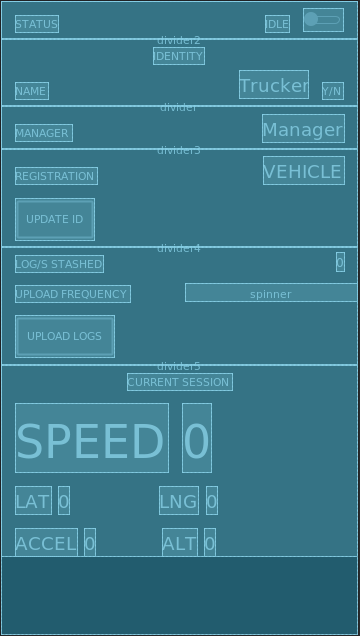
\includegraphics[scale=0.65]{android_ui.png}
\caption{Android Application - \ac{ui}}
\label{fig:android_ui}
\end{figure}

To account for different screen sizes, a Constraint layout is used, in which elements are tied to edges or specific points in the layout's geometry.
Elements are places relative to each other, and will dynamically adjust when tilting the screen.
The constraint layout is placed within a scroll view to allow scrolling if the elements can not fit on the screen.

The \ac{ui} allows the user to toggle the tracking service.
It provides information about the trucker and his/her manager.
An interface is provided for toggling upload frequency of logs.
Finally, the current sensor readings are displayed.

\subsubsection{Web Application}
\begin{figure}
\centering
    \subfigure[Fleet index page]
    {
        \centering
        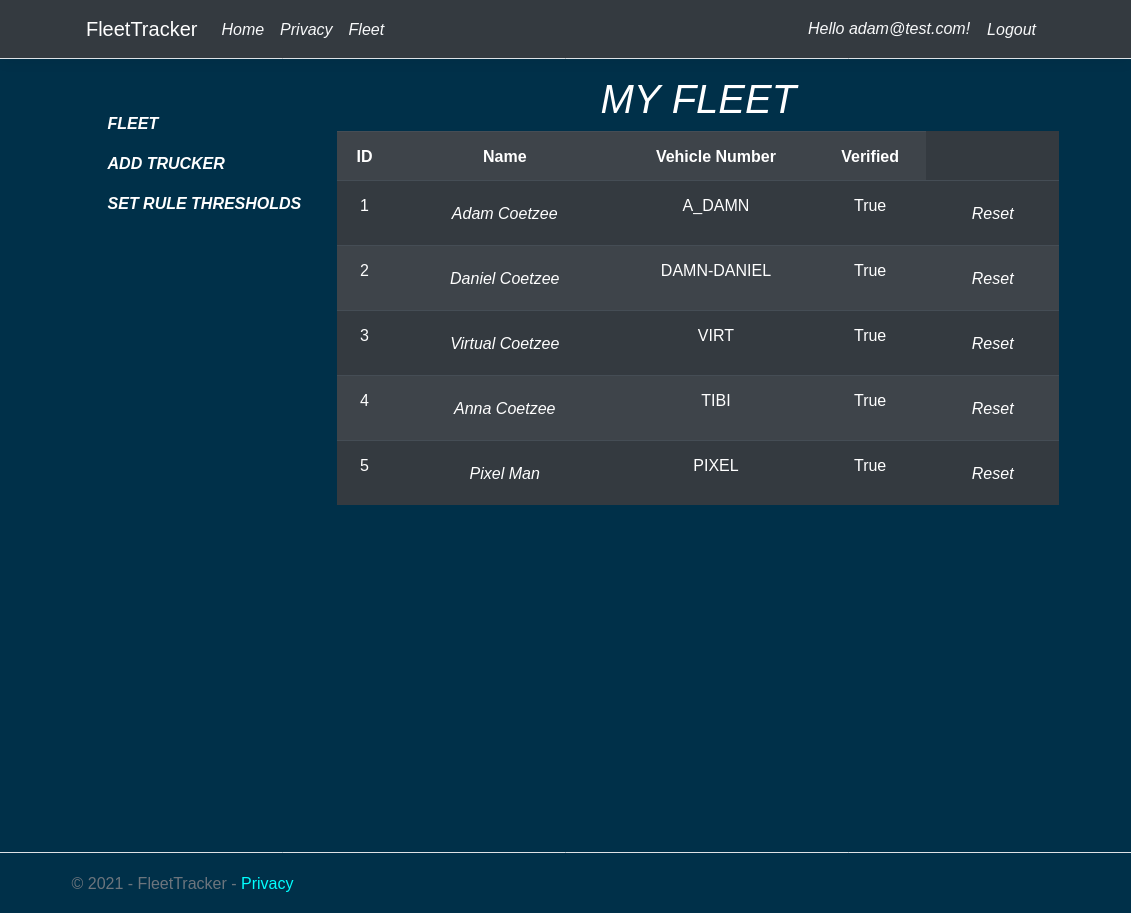
\includegraphics[width=2.5in]{fleet_index.png}
        \label{fig:fleet_index}
    }
    \subfigure[Add Trucker]
    {
        \centering
        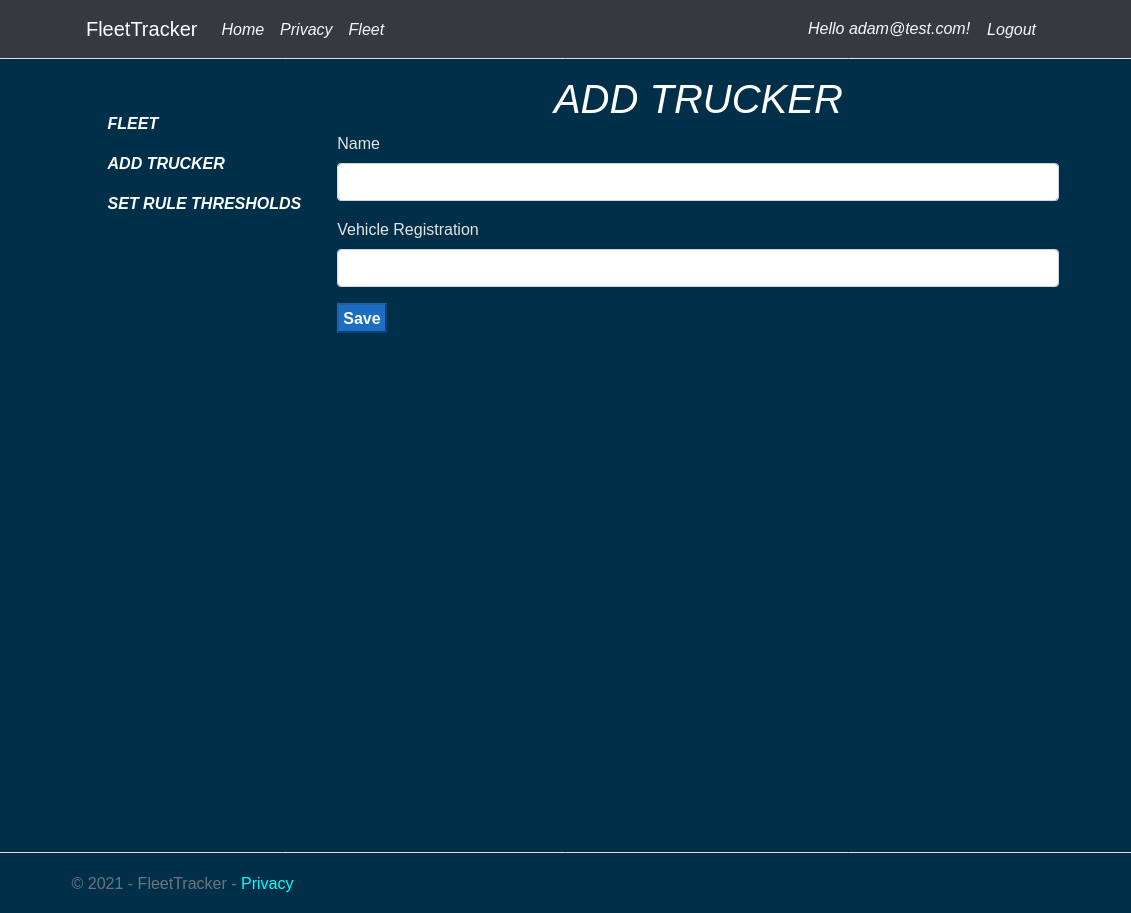
\includegraphics[width=2.5in]{fleet_add_trucker.png}
        \label{fig:fleet_add_trucker}
    }\\
    \subfigure[Set rules]
    {
        \centering
        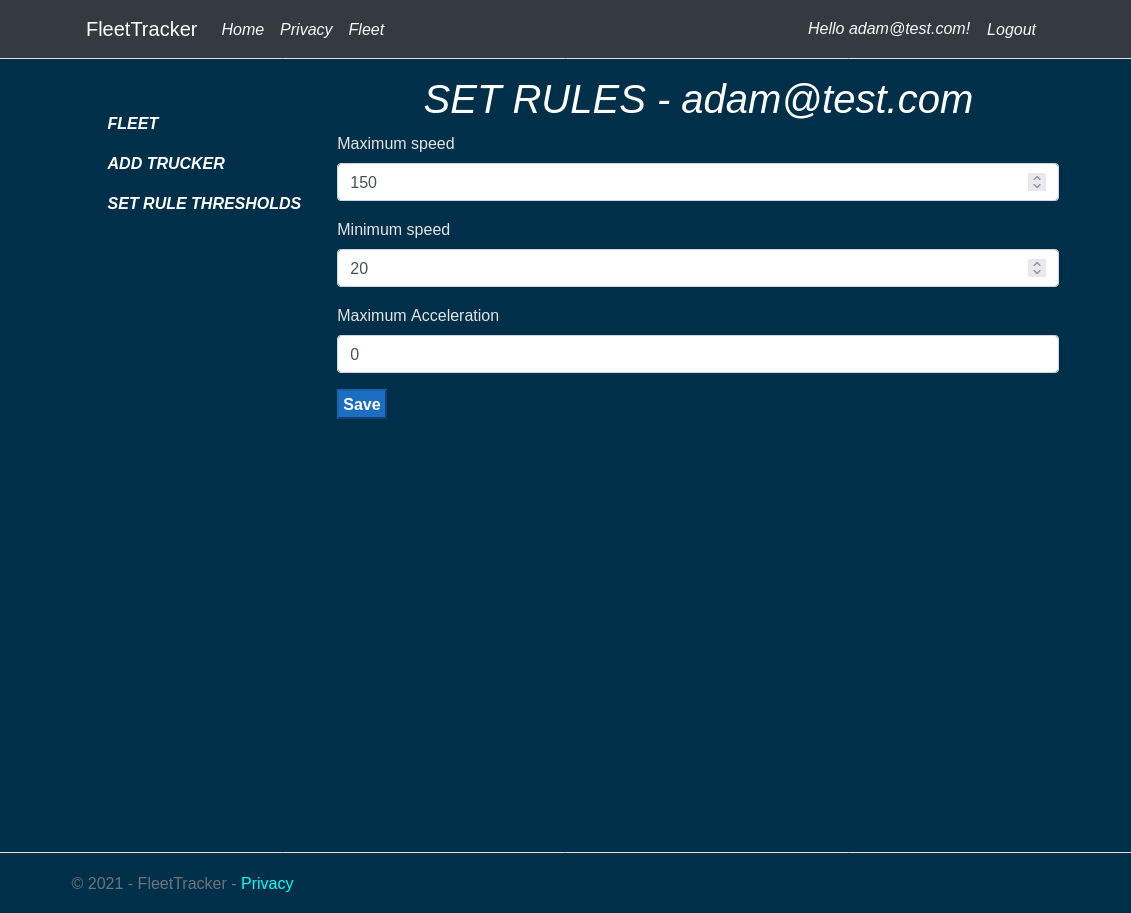
\includegraphics[width=2.5in]{fleet_set_rules.png}
        \label{fig:fleet_set_rules}
    }
    \subfigure[View Trucker]
    {
        \centering
        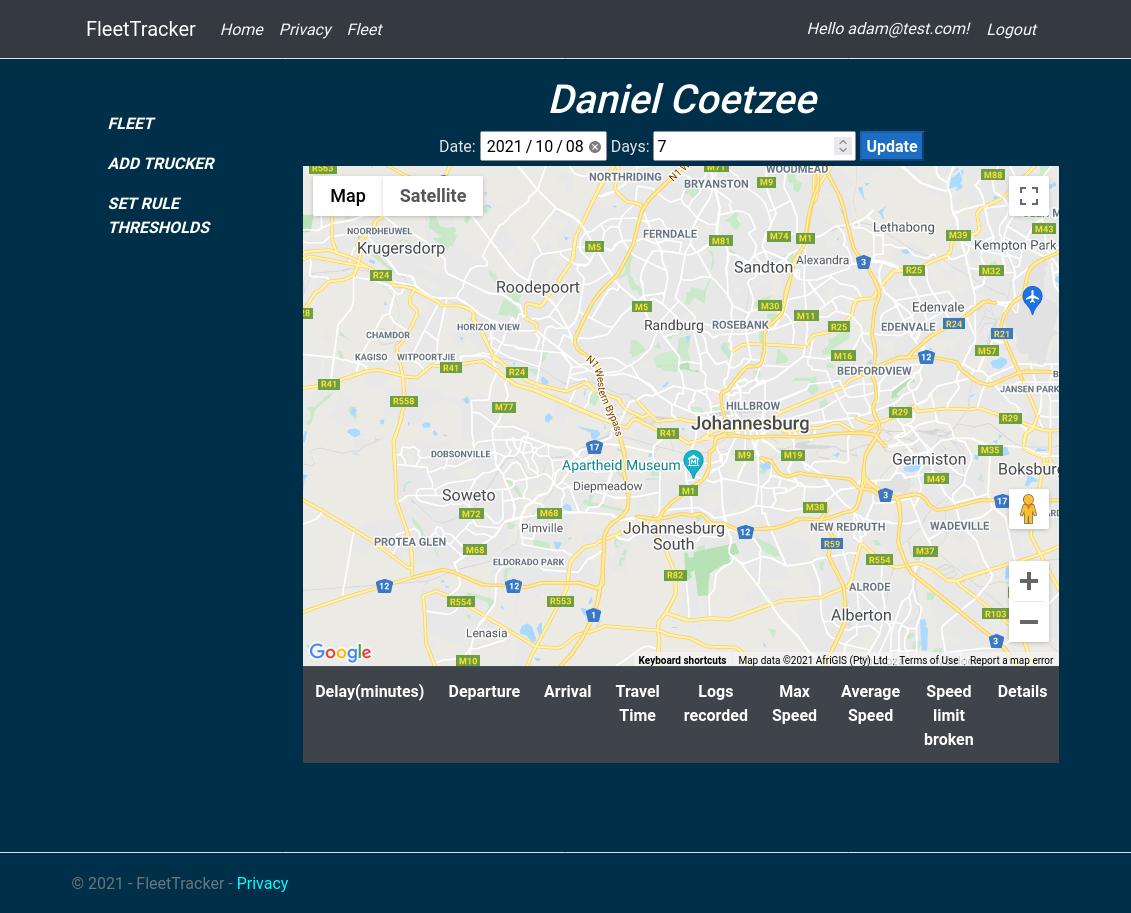
\includegraphics[width=2.5in]{fleet_view_trucker.png}
        \label{fig:fleet_view_trucker}
    }\\
    \subfigure[View Trip]
    {
        \centering
        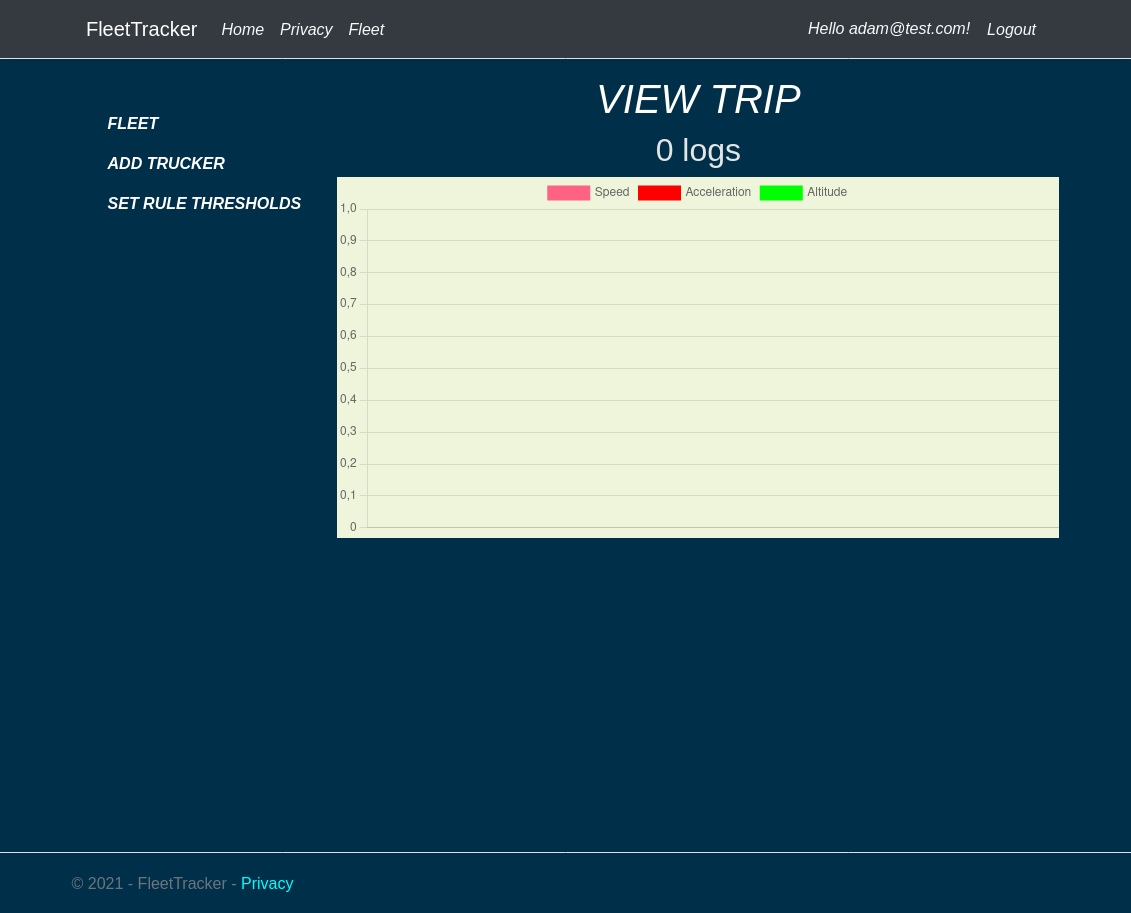
\includegraphics[width=2.5in]{fleet_view_trip.png}
        \label{fig:fleet_view_trip}
    }
\caption{Web application - Pages}
\label{fig:web_app_pages}
\end{figure}

Figure \ref{fig:web_app_pages} depicts the main pages used by managers for manipulating and viewing their fleets.
The web pages are designed using \ac{html} elements, which are style in \ac{css} aided by the \textit{Bootstrap} library which provides elegant \ac{css} presets.

\Ac{html} elements are spaced using \textit{div} containers in a grid layout.

\begin{itemize}
\item The index page, seen in figure \ref{fig:fleet_index} displays a list of truckers in the managers fleet. Managers can reset trucker \ac{id}s and navigate to individual trucker pages.
\item The "Add Trucker" page, in figure \ref{fig:fleet_add_trucker} allows managers to add new trucker entries.
\item The "Set Rules" page in figure \ref{fig:fleet_set_rules} allows managers to set rule thresholds for defining good behavior.
\item The "View Trucker" page, in figure \ref{fig:fleet_view_trucker} displays a map and table for displaying information about trips.
\item The "View Trip" page, in figure \ref{fig:fleet_view_trip} contains a graph for viewing statistics for trips.
\end{itemize}

\pagebreak
